\documentclass{article}
\usepackage[xetex]{graphicx}
\usepackage[slovak]{babel}
\usepackage{hyperref}
\hypersetup{
	colorlinks=true,
	linkcolor=blue,
	}
\title{Hannibal Barkas}
\author{Adam Jenča}
\begin{document}
\maketitle
\begin{center}
\hrule
\medskip
\center
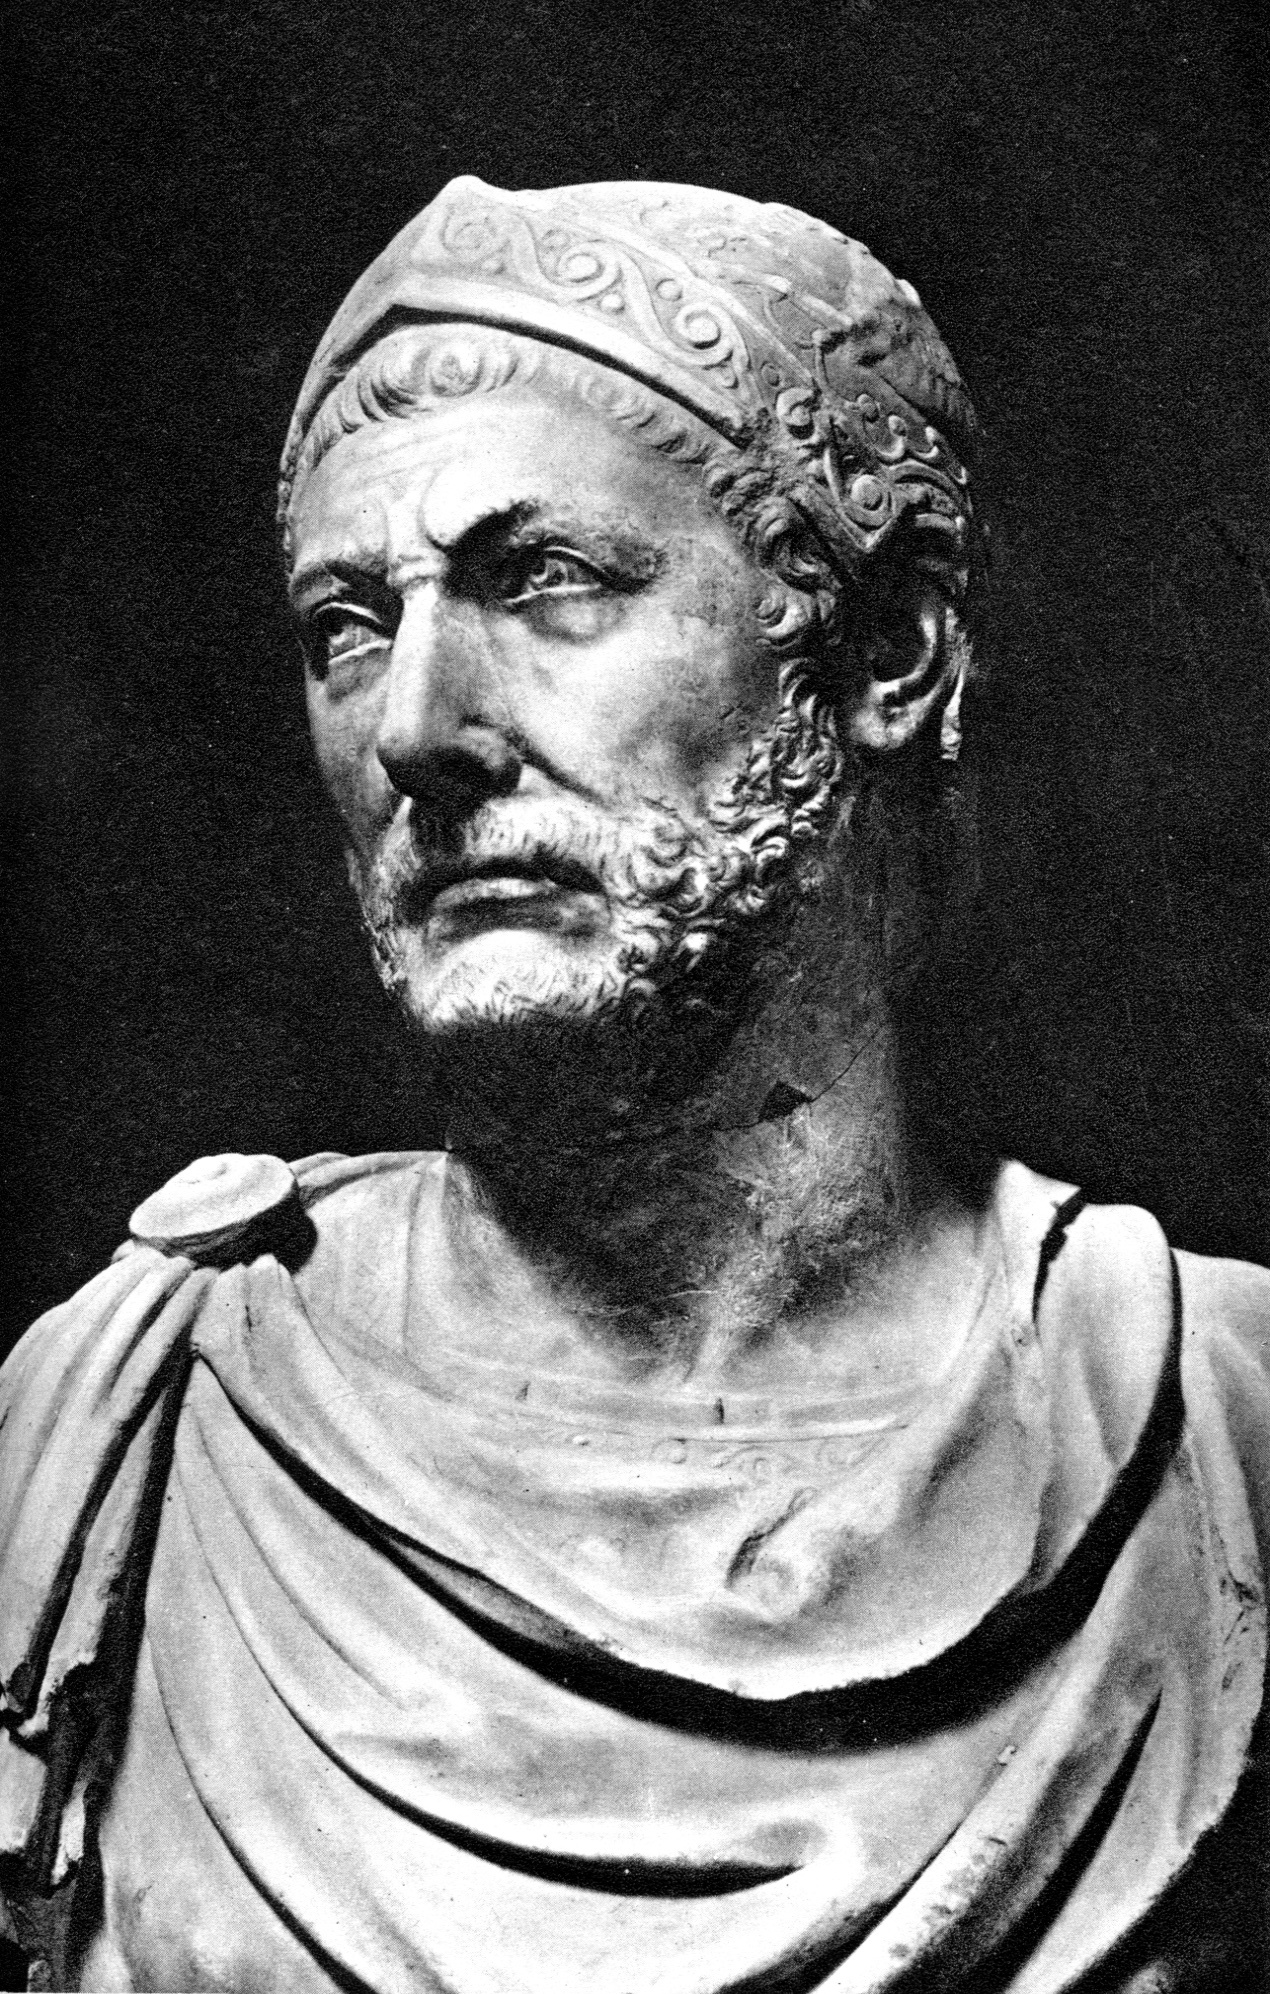
\includegraphics[scale=0.5]{hannibal_busta.jpg}
\end{center}
\newpage

\tableofcontents
\bigskip
\section{Úvod}

\textbf{Hannibal Barkas} bol kartáginský politik, štátnik a vojvodca\\
uznávaný najmä za svoje \textbf{strategické schopnosti}. \\
Preslávil sa 
\hyperref[subsubsec:alpine]{\textbf{prechodom cez Alpy}} počas 
\hyperref[subsec:secondpunianwar]{\textbf{Druhej Púnskej vojny}.}\\\\
\noindent
\section{Život}
\label{sec:life}
Narodil sa v roku \textbf{247 pred Kr.} vojvodcovi Hamilkarovi Barkasovi.\\
Ako deväťročný prisahal, že nikdy nebude sympatizovať s Rímom.
Už zamlada bol jeden z najlepších medzi jazdcami aj pešiakmi a vždy ako  prvý išiel do boja a ako posledný z neho odchádzal.
\subsection{Druhá púnska vojna}
\label{subsec:secondpunianwar}
Druhá púnska vojna bola druhá z rozsiahlych vojen medzi Kartágom a Rímom.
Hannibal v nej skoro dobyl Rím, ale poslali ho brániť rodné Kartágo.\\\\
\subsubsection{Cesta cez Alpy}
\label{subsubsec:alpine}
Rimania považovali Alpy za bezpečnú hranicu svojho územia. \\Hannibal teda spravil neočakávanú vec: s 80 000 pešiakmi, 12 000 jazdcami a 37 bojovými slonmi \\prešiel cez Pyreneje a cez Alpy, čím presunul vojnu do Ríma.
\\Cez Pyreneje prešiel ešte celkom ľahko a dostal sa do Galie. \\
Väčšinu domorodých kmeňov, ktoré s ním bojovali rozprášil, ale čast jeho bojovníkov sa zľakla polonahých Keltov a utiekla.\\
Od Keltov sa síce dozvedel, ako najbezpečnejšie prejsť cez Alpy, a1e Kartáginci boli zvyknutí skôr na púšte a nikdy predtým nevideli sneh.\\
Za 33 dní stratil 33 000 mužov. Nevedel slony prinútiť prejsť cez rieku, tak poranil najdivšieho slona a ostatné ho nasledovali.\\
\subsubsection{Bitka pri Ticine(218 pred Kr.)}
Keď Hannibal prekonal Alpy, pokúsil sa ho zastaviť Publius Cornelius Scipio, ale dobehol ho až pri rieke Ticine.
K boju došlo, keď sa stretli prieskumné skupiny oboch vojsk. 
Počas bitky bol Scipio zranený a jeho vojsko ustupovalo.
Scipia zachránil jeho syn, ktorý neskôr vyhral nad Hannibalom.
\begin{figure}
\center
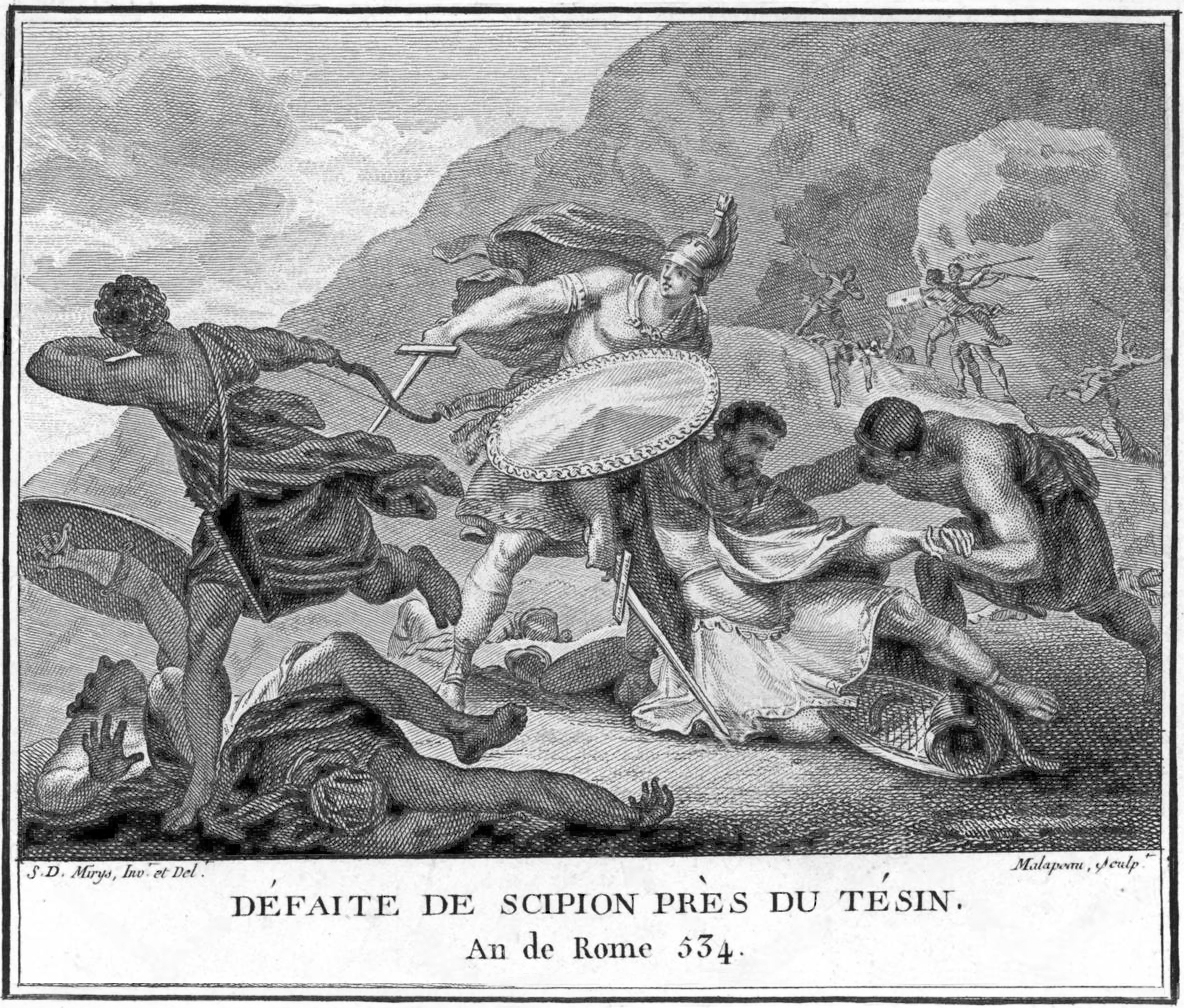
\includegraphics[scale=0.2]{ticinus.jpg}
\caption{Bitka pri Ticine}
\end{figure}
\newpage
\subsubsection{Bitka pri Trebii(218 pred Kr.)}
Po bitke pri Ticine Scipio prikázal, aby sa vojsko stiahlo po drevenom moste cez rieku Pád, a ut8borili sa v meste Placentia.\\Hannibal sa však o tom dosvedel prineskoro. Zdržalo ho aj to, že musel hľadať vhodný brod cez Pád. Údajne vytvoril zo slonov akúsi hrádzu. O niekoľko dní prišlo jeho vojsko k Placentii. V noci galské oddiely napadli stráže otvorili si brány a prebehli k Hannibalovi. Scipio sa obával, že by mohli napadnúť celé jeho vojsko, tak radšej prešiel cez Pád a založil nový tábor na brehu rieky. Kým Hannibal presunul vojakov a pritiahol k Scipiovmu táboru, zo Sicílie prišiel druhý konzul Tiberius Sempronius. Scipio nechcel bojovať, pretože bol zranený, ale jeden z menších rímskych oddielov prekvapil numídskych bojovníkov a rozprášil ich, čo Scipiovi dodalo odvahy. Hannibal s bratom Magonom pripravil na rímskych vojakov pascu: Časť numídskych bojovníkov vyprovokovala rímskych vojakov na druhý breh rieky. Vojaci boli premočení, lebo sa až po prsia brodili studenou vodou rieky Trebie. Hannibal zatiaľ pokojne rozmiestnil svojich bojovníkov. Premočení a  premrznutí Rimania sa čoskoro dostali do problémov. Kone sa splašili, lebo zacítili neznámy pach slonov.Rímska jazda sa horko-ťažko prebila cez stred vojska a stiahla sa späť do Placentie
\begin{figure}
\center
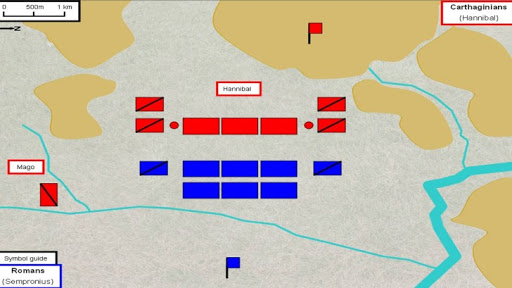
\includegraphics[scale=0.5]{trebius.jpg}
\caption{Bitka pri Trebii}
\end{figure}

\end{document}
